\input{preamble}

\begin{document}

\header{1}{Ray Tracing}
\setcounter{section}{-1}

In our first homework, we are going to implement a simple ray tracer (almost) from scratch.
We will provide some utility code such as the vector class and parallel threading. 
However, you will have to implement the rest yourself. Trust me, it will be fun!

Our homeworks are mostly inspired by the book \href{https://raytracing.github.io/}{Ray Tracing in One Weekend (RTOW)} (click the link for free access of the e-book). You are expected to read the relevant chapters of the book before implementing your own version. The structure of the homeworks is also largely inspired by \href{https://cs87-dartmouth.github.io/Fall2022/assignments.html}{CS 87/287 at Dartmouth} designed by Wojciech Jarosz (a UCSD alumni!).

Before you started coding, we recommend you to go through the whole handout to have some ideas of what needs to be done.

\paragraph{Coordinate systems conventions.} This is the most annoying part of any graphics systems as every single one of them use a different one. We will follow the conventions used in RTOW: Y axis is up, negative Z looks into the screen from the viewer, and we use a right-handed coordinate system.

\paragraph{Links in this document.} Some of the links in this document contain hyperlinks with a \emph{named anchor} to a webpage (e.g., \url{https://raytracing.github.io/books/RayTracingInOneWeekend.html\#overview}). On some PDF readers, I have found these links to not work very well (Adobe Acrobat Reader works well). If you encounter issues with the links, try replacing \lstinline{%23} with \lstinline{#} in the address bar of your browser.

\section{Building Torrey}
We are going to build our code on top of (a currently very barebone) renderer \emph{torrey}. Torrey already includes all the third party libraries (pugixml, pcg, stb\_image, tinyexr, miniz, tinyply) in its repo and all you need to do is to clone the repo and build it using CMake (assuming you are in a Unix-like system):
\begin{lstlisting}[language=bash]
  git clone https://github.com/BachiLi/torrey_public
  mkdir build
  cd build
  cmake ..
  make -j
\end{lstlisting}

After building, you should see an executable \lstinline{torrey}. Try typing the following command:
\begin{lstlisting}[language=bash]
  torrey -hw 1_1
\end{lstlisting}
It will generate an image \lstinline{hw_1_1.exr} that looks like Figure~\ref{fig:hw_1_1_before}:
\begin{figure}[ht]
    \centering
    \includegraphics[width=0.5\linewidth]{imgs/hw_1_1_before.png}
    \caption{Image output by the homework 1.1 code before your modification.}
    \label{fig:hw_1_1_before}
\end{figure}

\lstinline{.exr} is an image format that is suitable for storing \emph{high-dynamic range} images. Basically, instead of storing 8-bit (0-255) per color channel, we store a floating point number per channel. To view \lstinline{.exr}, I recommend using \href{https://github.com/wkjarosz/hdrview}{HDRView} or \href{https://github.com/Tom94/tev}{Tev}.

Read \lstinline{main.cpp}, \lstinline{hw1.cpp}, \lstinline{vector.h}, and \lstinline{image.h} to understand the current code structure.

\section{Sending rays from the camera}
To do ray tracing, we need to first shoot rays from the camera. In this first step, we will generate camera rays for all the pixels. The goal of our first task is to visualize the camera ray direction (normalized to unit length per pixel).

First, read \href{https://raytracing.github.io/books/RayTracingInOneWeekend.html\#rays,asimplecamera,andbackground}{Chapter 4.2} of the first RTOW book and understand its content.

We will use a very simple perspective camera for now. The position is fixed at $(0, 0, 0)$, and the camera is facing towards $(0, 0, -1)$ with an up vector $(0, 1, 0)$, right vector $(1, 0, 0)$, and focal length of $1$ (the same setting as the ROTW book). We will make the camera ``positionable'' later. For each pixel, we will shoot a ray from the center of the pixel (for a pixel $(x, y) \in [0, \text{width}] \times [0, \text{height}]$, we shoot a ray in $(x + 0.5, y + 0.5)$). Go to \lstinline{hw1.cpp} and look at the function \lstinline{hw_1_1}. Your task is to modify the function to output the \emph{unit length} ray direction per pixel. Some of the pixels will have negative color but that is fine. See Figure~\ref{fig:hw_1_1_after} \lstinline{handouts/imgs/hw_1_1.exr} for references.

Don't worry about the \lstinline{params} argument of the function. We will use it in the later part.

You may find the \lstinline{normalize} function in \lstinline{vector.h} to be useful.

To see your results, in terminal, type
\begin{lstlisting}[language=bash]
  torrey -hw 1_1
\end{lstlisting}

\begin{figure}[ht]
    \centering
    \includegraphics[width=0.5\linewidth]{imgs/hw_1_1_after.png}
    \caption{Image output by the homework 1.1 code after your modification.}
    \label{fig:hw_1_1_after}
\end{figure}

\paragraph{Quiz:} How do you modify your code to render using a camera with 360 degree field of view like Figure~\ref{fig:360_camera}? (hint: see \href{https://en.wikipedia.org/wiki/Spherical_coordinate_system}{spherical coordinates}) Briefly describe your approach (you can attach your code if you want).
\begin{figure}[ht]
    \centering
    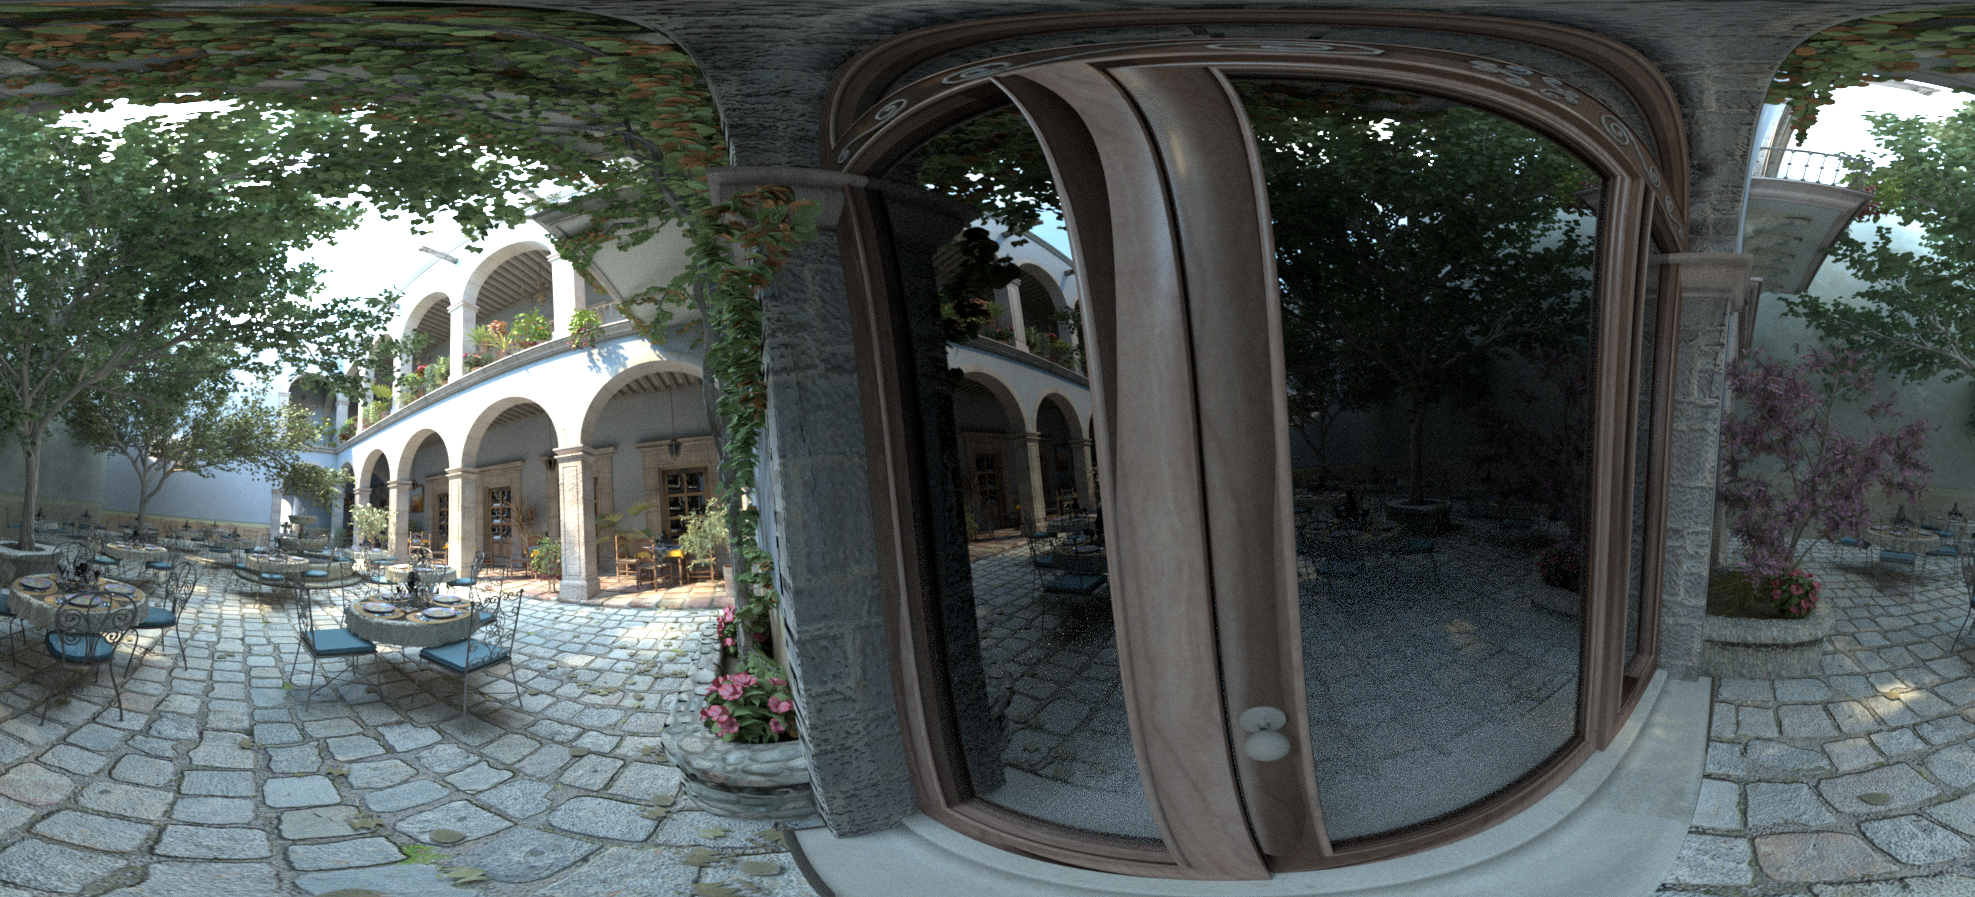
\includegraphics[width=0.5\linewidth]{imgs/360camera.png}
    \caption{360 camera rendering taken from the \href{https://www.pbr-book.org/3ed-2018/Camera_Models/Environment_Camera}{PBRT book}.}
    \label{fig:360_camera}
\end{figure}

\section{Intersection with one sphere}
After we have the rays from the camera, we'll trace these rays and intersect them with the scene. Here we choose the geometry to be a sphere (because it's easy and we can easily build interesting scenes using only spheres). For this part, let's try to handle only one sphere.

First, read \href{https://raytracing.github.io/books/RayTracingInOneWeekend.html\#addingasphere}{Chapter 5} and \href{https://raytracing.github.io/books/RayTracingInOneWeekend.html\#surfacenormalsandmultipleobjects}{Chapter 6} of RTOW and understand the content.

Next, go to \lstinline{hw1.cpp} and look at the function \lstinline{hw_1_2}. Your task is to modify the function to output the surface normal of the sphere. The sphere has unit radius and is located at $(0, 0, 2)$. The camera pose is exactly the same as the previous part. To make prettier images this time, let's map the normal to positive numbers: for a 3D vector $n$, we map it to the final color $c = \frac{n + 1}{2}$. If our rays do not hit the sphere, return $(0.5, 0.5, 0.5)$.

You may find the struct \lstinline{hw1::SpherePrimitive} in \lstinline{hw1_scenes.h} to be helpful, but you are not required to use it.

You may also find the \lstinline{infinity} function in \lstinline{torrey.h} to be useful.

To see your results, in terminal, type
\begin{lstlisting}[language=bash]
  torrey -hw 1_2
\end{lstlisting}

The results generated from our code looks like Figure~\ref{fig:hw_1_2}:
\begin{figure}[ht]
    \centering
    \includegraphics[width=0.5\linewidth]{imgs/hw_1_2.png}
    \caption{Your homework 1.2 should output this image.}
    \label{fig:hw_1_2}
\end{figure}

\paragraph{Quiz:} If we were to add a linear transformation to the sphere (e.g., turn it into an ellipsoid), how would you do it? Briefly describe your approach.

\section{Adding camera control}
We will next add pose and field of view control to the camera so that we can look at the sphere at different angles. We will adopt the LookAt transform since it's more intuitive. We will also follow RTOW and take a vertical field of view angle.

First, read \href{https://raytracing.github.io/books/RayTracingInOneWeekend.html#positionablecamera}{Chapter 11} of RTOW and understand the content.

Next, go to \lstinline{hw1.cpp} and look at the function \lstinline{hw_1_3}. Given the inputs \lstinline{lookfrom}, \lstinline{lookat}, \lstinline{up}, \lstinline{vfov} (we have parsed it for you from the command line arguments \lstinline{params}), transform your camera rays accordingly and render the same sphere in \lstinline{hw_1_2}.

You may find the \lstinline{radians} function in \lstinline{torrey.h} to be useful.

To see your results, in terminal, type
\begin{lstlisting}[language=bash]
  torrey -hw 1_3 -lookfrom 1 0 -1 -lookat 0 0 -2 -vfov 60
  torrey -hw 1_3 -lookfrom 0 0 -0.75 -lookat 0 0 -2 -vfov 90
  torrey -hw 1_3 -lookfrom 1 -1 0 -lookat 1 -1 -2 -vfov 90
  torrey -hw 1_3 -lookfrom 1 -1 1 -lookat 1 -1 -2 -vfov 45
\end{lstlisting}
or just any parameter you like! See Figure~\ref{fig:hw_1_3} for references.

\begin{figure}[ht]
    \centering
    \includegraphics[width=0.24\linewidth]{imgs/hw_1_3a.png}
    \includegraphics[width=0.24\linewidth]{imgs/hw_1_3b.png}
    \includegraphics[width=0.24\linewidth]{imgs/hw_1_3c.png}
    \includegraphics[width=0.24\linewidth]{imgs/hw_1_3d.png}
    \caption{References for Homework 1.3.}
    \label{fig:hw_1_3}
\end{figure}

\paragraph{Quiz:} If we were to specify the \emph{horizontal} field of view angle instead of the vertical one, how should we rewrite the code?

\paragraph{Quiz:} In the RTOW book, to compute the coordinate frame for the camera rays (\lstinline{w, u,} and \lstinline{v}), their code normalizes the cross product of the \lstinline{up} vector and the \lstinline{w} vector. However, when they do the cross product between \lstinline{w} and \lstinline{u}, the result did not need to be normalized. Why?

\paragraph{Quiz:} Compare the third and fourth images in Figure~\ref{fig:hw_1_3}. Why is the sphere in the third image more \emph{distorted} compared to the fourth image? (Hint: you may want to read \href{https://en.wikipedia.org/wiki/Perspective_distortion}{this} Wikipedia article.)

\section{Intersection with many spheres}
Next, we will extend our ray tracer to handle multiple spheres in the scene. Take your code from the previous part, and add a for loop to intersect with all the spheres. This part should be much easier than the previous one. 

Go to \lstinline{hw1.cpp} and modify the function \lstinline{hw_1_4}. We will use the command line argument \lstinline{params} to access the scenes. Use \lstinline{hw1_scenes[scene_id]} to access your scene. The scene is contained in the struct \lstinline{hw1::Scene}, defined in \lstinline{hw1_scenes.h}:
\begin{lstlisting}[language=C++]
struct Scene {
    Camera camera;
    std::vector<SpherePrimitive> primitives;
    std::vector<PointLight> lights; 
};
\end{lstlisting}
Ignore the lights for now. We will use them later. Also don't worry about \lstinline{back_diffuse_color} just now.
After you intersect the spheres, instead of outputting the normal, let's output the \lstinline{diffuse_color} of the sphere this time. As usual, if our rays do not hit any sphere, return $(0.5, 0.5, 0.5)$.

To see your results, in terminal, type
\begin{lstlisting}[language=bash]
  torrey -hw 1_4 [scene_id]
\end{lstlisting}
where \lstinline{[scene_id]} is the scene you want to render (0-4).

Figure~\ref{fig:hw_1_4} shows our renderings for the five scenes.

\begin{figure}[ht]
    \centering
    \includegraphics[width=0.19\linewidth]{imgs/hw_1_4a.png}
    \includegraphics[width=0.19\linewidth]{imgs/hw_1_4b.png}
    \includegraphics[width=0.19\linewidth]{imgs/hw_1_4c.png}
    \includegraphics[width=0.19\linewidth]{imgs/hw_1_4d.png}
    \includegraphics[width=0.19\linewidth]{imgs/hw_1_4e.png}
    \caption{References for Homework 1.4.}
    \label{fig:hw_1_4}
\end{figure}

By the way, if you are interested of how the last scene is authored, it is generated by the following Python script:
\begin{lstlisting}[language=Python]
import numpy as np
n = 30
center = 5 * np.random.rand(3, n) - 2.5
center[2,:] -= 5
radius = (np.random.rand(1, n) + 0.5) / 2
color = np.random.rand(3, n)
for i in range(n):
    print(f'{{Vector3{{{center[0,i]:.3f},{center[1,i]:.3f},{center[2,i]:.3f}}}, {radius[0, i]:.3f}, Vector3{{{color[0,i]:.3f},{color[1,i]:.3f},{color[2,i]:.3f}}}}},')
\end{lstlisting}

\section{Lighting with point lights and Lambertian surfaces}
Rendering with constant color is a bit boring. Let's add some variation to the color. For each scene, we have a list of point lights, and we are going to compute the influence of these lights to our spheres.

Here is where we slightly deviate from RTOW (RTOW doesn't introduce the notion of lights until the end of the second book, which I find to be a bit late). Given a list of lights and a point hit by our camera ray (we usually call it the \emph{shading point}), we will compute the following response:
\begin{equation}
    \sum_{\text{light}} \frac{\max\left(n \cdot l, 0\right)}{\pi} \cdot \frac{I}{d^2} \cdot K_d \cdot \text{visibility},
    \label{eq:lighting}
\end{equation}
where $n$ is the normal of the surface, $l$ is the normalized vector between the shading point and the point light position, $I$ is the intensity of the light, $d$ is the distance between the shading point and the light, $K_d$ is the \lstinline{diffuse_color} of the surface (it is also called \emph{albedo} or \emph{diffuse reflectance}), $\text{visibility}$ is $1$ if the shading point can see the light and is $0$ otherwise. In practice this means you need to shoot a \emph{shadow ray} to test whether the light is blocked by your shading point. You can reuse your previous intersection functions to compute $\text{visibility}$.

\paragraph{Quiz:} explain the equation above -- Why is there a dot product? Why is there a distance square? Don't worry about the $\pi$ too much. It will make sense when we talk about BRDFs in the class.

Go to \lstinline{hw1.cpp} and modify the function \lstinline{hw_1_5}. As usual, use \lstinline{hw1_scenes[scene_id]} to access your scene. After you intersect the spheres, compute Equation~\eqref{eq:lighting} above.

\paragraph{Shadow epsilon.} When doing the shadow ray test, you may find that due to the finite precision of float points, the test can accidentally mark the sphere on the shading point as occluding itself. Robustly resolving this problem is tricky, but there is an easy hack: we can set the \lstinline{tmin} and \lstinline{tmax} of our shadow ray to be $\epsilon$ and $\left(1 - \epsilon\right) d$ respectively, where $\epsilon$ is a small number. For now, let's set $\epsilon = 10^{-4}$ (ideally, $\epsilon$ should be proportional to the scale of the scene, but let's not worry about that right now).

\paragraph{Front facing vs back facing normals.} Read \href{https://raytracing.github.io/books/RayTracingInOneWeekend.html#surfacenormalsandmultipleobjects/frontfacesversusbackfaces}{Chapter 6.4} of RTOW and have an understanding of the difference between front facing and back facing normals. In our rendering system, we assign two different materials to the front facing part of the surface and the back facing part. If your ray hit the front facing part, use \lstinline{diffuse_color}. On the other hand, if it hits the back facing part, use \lstinline{back_diffuse_color}. For the back facing normals, flip them during shading so that the dot product is not zero.

As usual, to see your results, in terminal, type
\begin{lstlisting}[language=bash]
  torrey -hw 1_5 [scene_id]
\end{lstlisting}
where \lstinline{[scene_id]} is the scene you want to render (0-4).

Figure~\ref{fig:hw_1_5} shows our renderings for the five scenes.

\begin{figure}[ht]
    \centering
    \includegraphics[width=0.19\linewidth]{imgs/hw_1_5a.png}
    \includegraphics[width=0.19\linewidth]{imgs/hw_1_5b.png}
    \includegraphics[width=0.19\linewidth]{imgs/hw_1_5c.png}
    \includegraphics[width=0.19\linewidth]{imgs/hw_1_5d.png}
    \includegraphics[width=0.19\linewidth]{imgs/hw_1_5e.png}
    \caption{References for Homework 1.5.}
    \label{fig:hw_1_5}
\end{figure}

\paragraph{Quiz:} Read about \href{https://en.wikipedia.org/wiki/Three-point_lighting}{three-point lighting} on Wikipedia. In the second scene (\lstinline{scene_id=1}), which light is the key light? Which light is the fill light? Which light is the backlight? Do you think this is better than only having the key light? Why?

\section{Antialiasing}
If you have been watching your images closely, you will find that they have some ugly jagged edges around object and shadow boundaries. The issue is that we always trace rays through the center of pixels. We can easily fix it by averaging the samples in the support of a pixel.

Go read \href{https://raytracing.github.io/books/RayTracingInOneWeekend.html#antialiasing}{Chapter 7} of RTOW.

Go to \lstinline{hw1.cpp} and modify the function \lstinline{hw_1_6}. As usual, use \lstinline{hw1_scenes[scene_id]} to access your scene. This time, we additionally take an argument \lstinline{-spp [spp]} that indicates how many \emph{samples per pixel} we will be using. We have parsed it for you. You will notice that the image resolution this time is a lot lower. We want to use this to show the effect of antialiasing. Try to compare to the previous renderings at the same resolution.

\paragraph{Random number generation.} Please do \emph{not} use the C \lstinline{rand()} function. It is really really really really bad: \lstinline{rand} usually have very short period as a random number generator (32768 in many systems), it uses a global variable to store the states of the random number generator, and this significantly hurts parallelization. Most implementations of \lstinline{rand} also use a bad random number generator (a very basic LCG). The modern C++ random number generator is much better, but not perfect. I personally prefer \href{https://www.pcg-random.org/}{PCG}. Highly recommend Melissa O'Neill's \href{https://www.youtube.com/watch?v=45Oet5qjlms}{talk} about PCG if you are interested in the topic of random number generation.

 
%\bibliographystyle{plain}
%\bibliography{refs}

\end{document}
